\subsection*{1.5 Kirchhoffsche Regeln}
    \subsubsection*{Knotenregel}
    \vspace{-1mm}
    \begin{minipage}{0.49\linewidth}
        \begin{footnotesize}
            \begin{center}
                \vspace{2mm}
                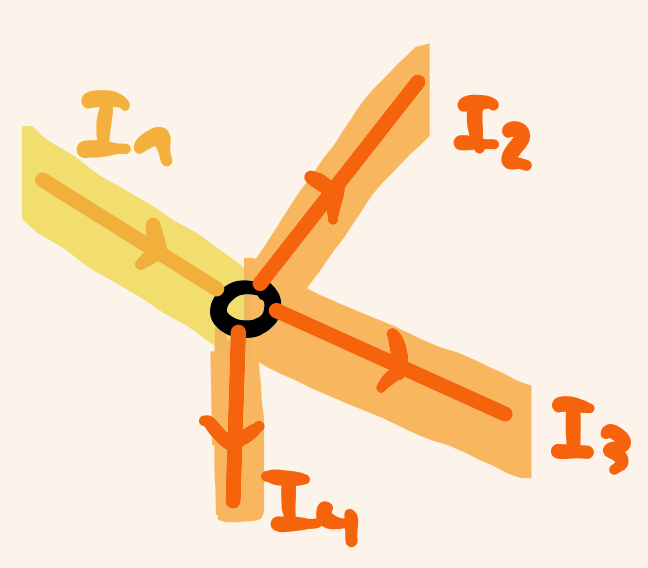
\includegraphics[width = 30mm]{src/images/knotenregel.png}
            \end{center}
        \end{footnotesize}
    \end{minipage}
    \begin{minipage}{0.5\linewidth}
        \begin{scriptsize}
            \begin{center}
                \mathbox{
                    \sum\limits_k I_k = 0
                }
            \end{center}
        \end{scriptsize}
    \end{minipage}
    \vspace{1mm}
    \hfill \colorbox{Goldenrod}{$\sum I_\text{zufliessend}$} $=$ \colorbox{Apricot}{$\sum I_\text{abfliessend}$} 


    \subsubsection*{Maschenregel}
    \vspace{-1mm}
    \begin{minipage}{0.49\linewidth}
        \begin{footnotesize}
            \begin{center}
                \vspace{2mm}
                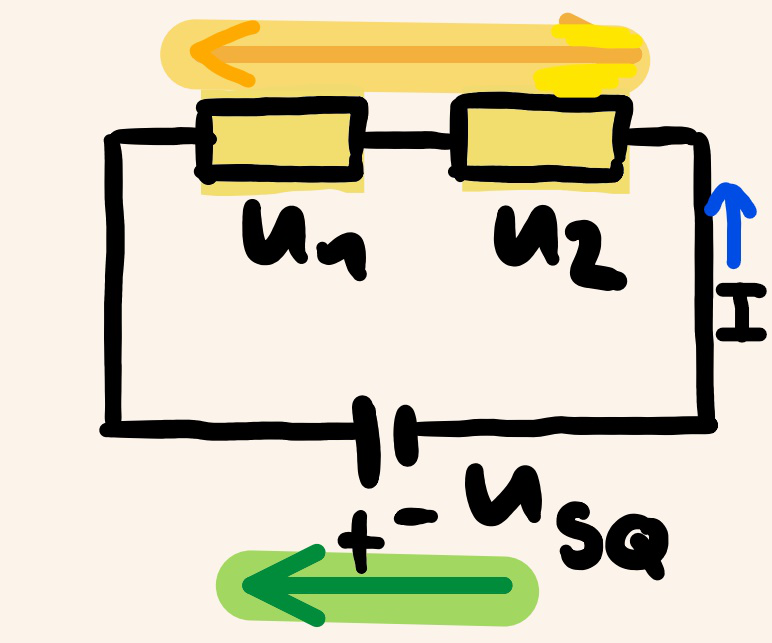
\includegraphics[width = 30mm]{src/images/maschenregel.png}
            \end{center}
        \end{footnotesize}
    \end{minipage}
    \begin{minipage}{0.5\linewidth}
        \begin{scriptsize}
            \begin{center}
                \mathbox{
                    \sum\limits_{sq} U_{sq} = \sum\limits_i U_i = \sum\limits_k R_k I_k 
                }
            \end{center}
        \end{scriptsize}
    \end{minipage}
    \vspace{1mm}
    \hfill \colorbox{YellowGreen}{$\sum U_\text{Spannungsquelle}$} $=$ \colorbox{Yellow}{$\sum U_\text{Spannungsabfälle}$} 

    (1) Zeichne \colorbox{YellowGreen}{$\overrightarrow{U_{sq}}$}an der Spannungsquelle ein (minus nach plus)
    \\(2) Wähle Stromrichtung \colorbox{Cyan}{$\overrightarrow{I}$} (gegen $U_{sq}$)
    \\(3) Trage \colorbox{Yellow}{$\overrightarrow{U_R}$} an Widerständen (ein gleich wie Stromrichtung)
    \vspace{20mm}